
\section{Introduction}
High Alfv\'enicity ($|\sigma_c| \rightarrow 1$ and $\sigma_r \rightarrow 0$) indicates \textbf{propagation of/propagating?} Alfv\'en waves \cite{Bavassano:1998}. Alfv\'en waves are electromagnetic waves in which ions oscillate along a magnetic field line at the Alfv\'en speed. 




\section{Data}
In order to ensure that the MMS probes were in the quasi-perpendicular region of the magnetosheath, only time periods in the list with $x_{GSE}>0\hspace{5pt}R_E$ and $y_{GSE}>0\hspace{5pt}R_E$. \citeA{ToyEdens2:2024} includes all MMS probes in their analysis; however, we only consider MMS-1 since presumably the other 3 MMS probes are in the same region. 107 time periods were obtained for this study from the Toy-Edens list 

% note: 107 periods were used for detection; however of the total events, 5 events overlapped with mine that I had already run and then there was 1 period with data not available and 3 with time periods not really inside the magnetosheath by visual identification of time series data



\section{Wavelet analysis}
This is because of the windowed analysis: as the maxima in reduced magnetic helicity are recorded in each window, there will be overlapping events identified. After all the windows are searched, the compiled event list is then processed to eliminate overlapping events.

by comparing two adjacently overlapping events and keeping the one with the highest maximum in $|\sigma_m|$. This is repeated until there are no overlapping events left.


\section{GS method}
The automated detection algorithm moves through different windowed periods of the data, with each window identifying events of certain duration. We employ windows with a minimum duration from approximately 30 seconds (10$\Delta t$) to a maximum duration of 343 data points, which corresponds to approximately 17 minutes for THEMIS data, and 25 min for MMS data. In order to identify two-dimensional magnetic structures from single-spacecraft data \citep{Paschmann:2008}, the \textit{\textit{in situ}} magnetic field and plasma data from a specified window of time are transformed into the co-moving frame, notably the de Hoffman-Teller frame \citep{deHoffman-Teller:1950}. Through a trial-and-error process to determine the optimal orientation of the $z$-axis, the azimuthal and poloidal angles that define this frame transformation are chosen. The azimuthal angle $\phi$ is the longitude of the FR $z$-axis, which measures the angle between the $x$-direction and the projection of the $z$-axis onto the $xy$-plane. The polar angle $\theta$ is the angle between the FR $z$-axis and the GSE $z$-direction. The azimuthal angle $\Phi$ is the rotational angle around the $z$-axis (in the $xy$-plane), and polar angle $\theta$ is the angle between the $z$-axis and the velocity vector of the spacecraft.

\section{Results}
Figures \ref{fig:histogram-orientation}, \ref{fig:histogram-flux}, and \ref{fig:histogram-helicitydensity} are distributions of parameters obtained from the GS-based algorithm only: orientation angles of the $z$-axis of the magnetic structures, local maximum of the scalar flux function $|A_m| = \textnormal{max}(|A(x,y)|)$, and the approximation to the helicity density per unit length.

\begin{figure}
    \centering
    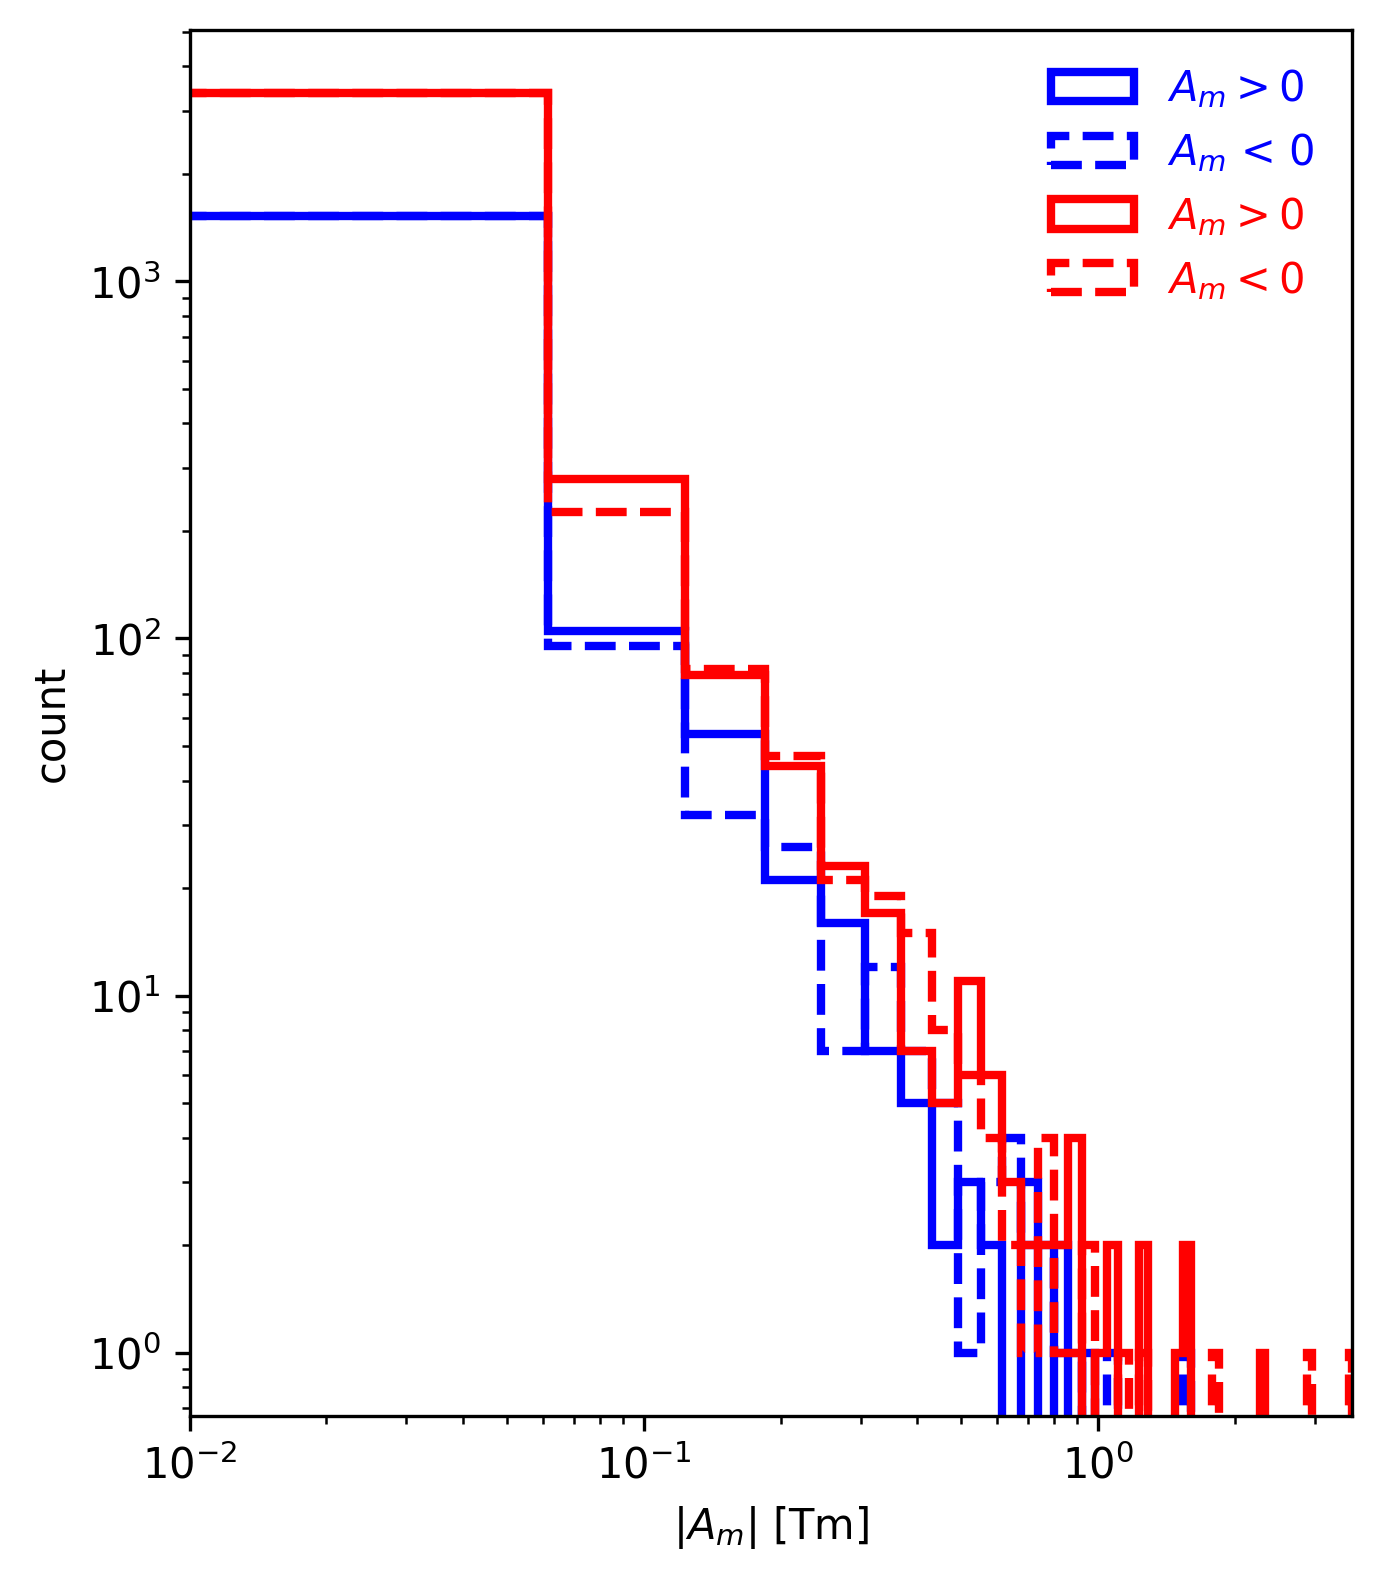
\includegraphics[width=0.6\textwidth]{Figures/Histograms/histogram_Asplit.png}
    \caption{Histograms for the local maximum magnetic flux $|A_m|$ of events identified via GS analysis. The blue lines represent events in the solar wind, and the red lines represent events in the magnetosheath. The dashed lines show where the poloidal magnetic flux per unit length is less than zero.}
    \label{fig:histogram-Asplit}
\end{figure}

The distribution of the proportionality constant $\alpha$ partially represents the data in Table \ref{tab:walenTest-table}. It can be seen that events with a high Alfv\'en Mach number (and thus proportionality constant $\alpha$) are more prominent in the magnetosheath. However, there is a higher relative amount of events with Wal\'en slope $|w|>0.3$ in the solar wind than in the magnetosheath. The mean $\alpha$ for events with $|w|\leq 0.3$ was 0.337 and 0.366 for the solar wind and magnetosheath, respectively. For $|w|>0.3$, the means had a greater difference at 0.059 and 0.139 for the respective regions. The median values for $\alpha$ in the solar wind were $7.575\times 10^{-3}$ for $|w|\leq 0.3$ and 0.297 for $|w|>0.3$. In the magnetosheath, the median values for $\alpha$ were 0.055 and 0.323 for $|w|\leq 0.3$ and $|w|>0.3$, respectively.

\begin{figure}
    \centering
    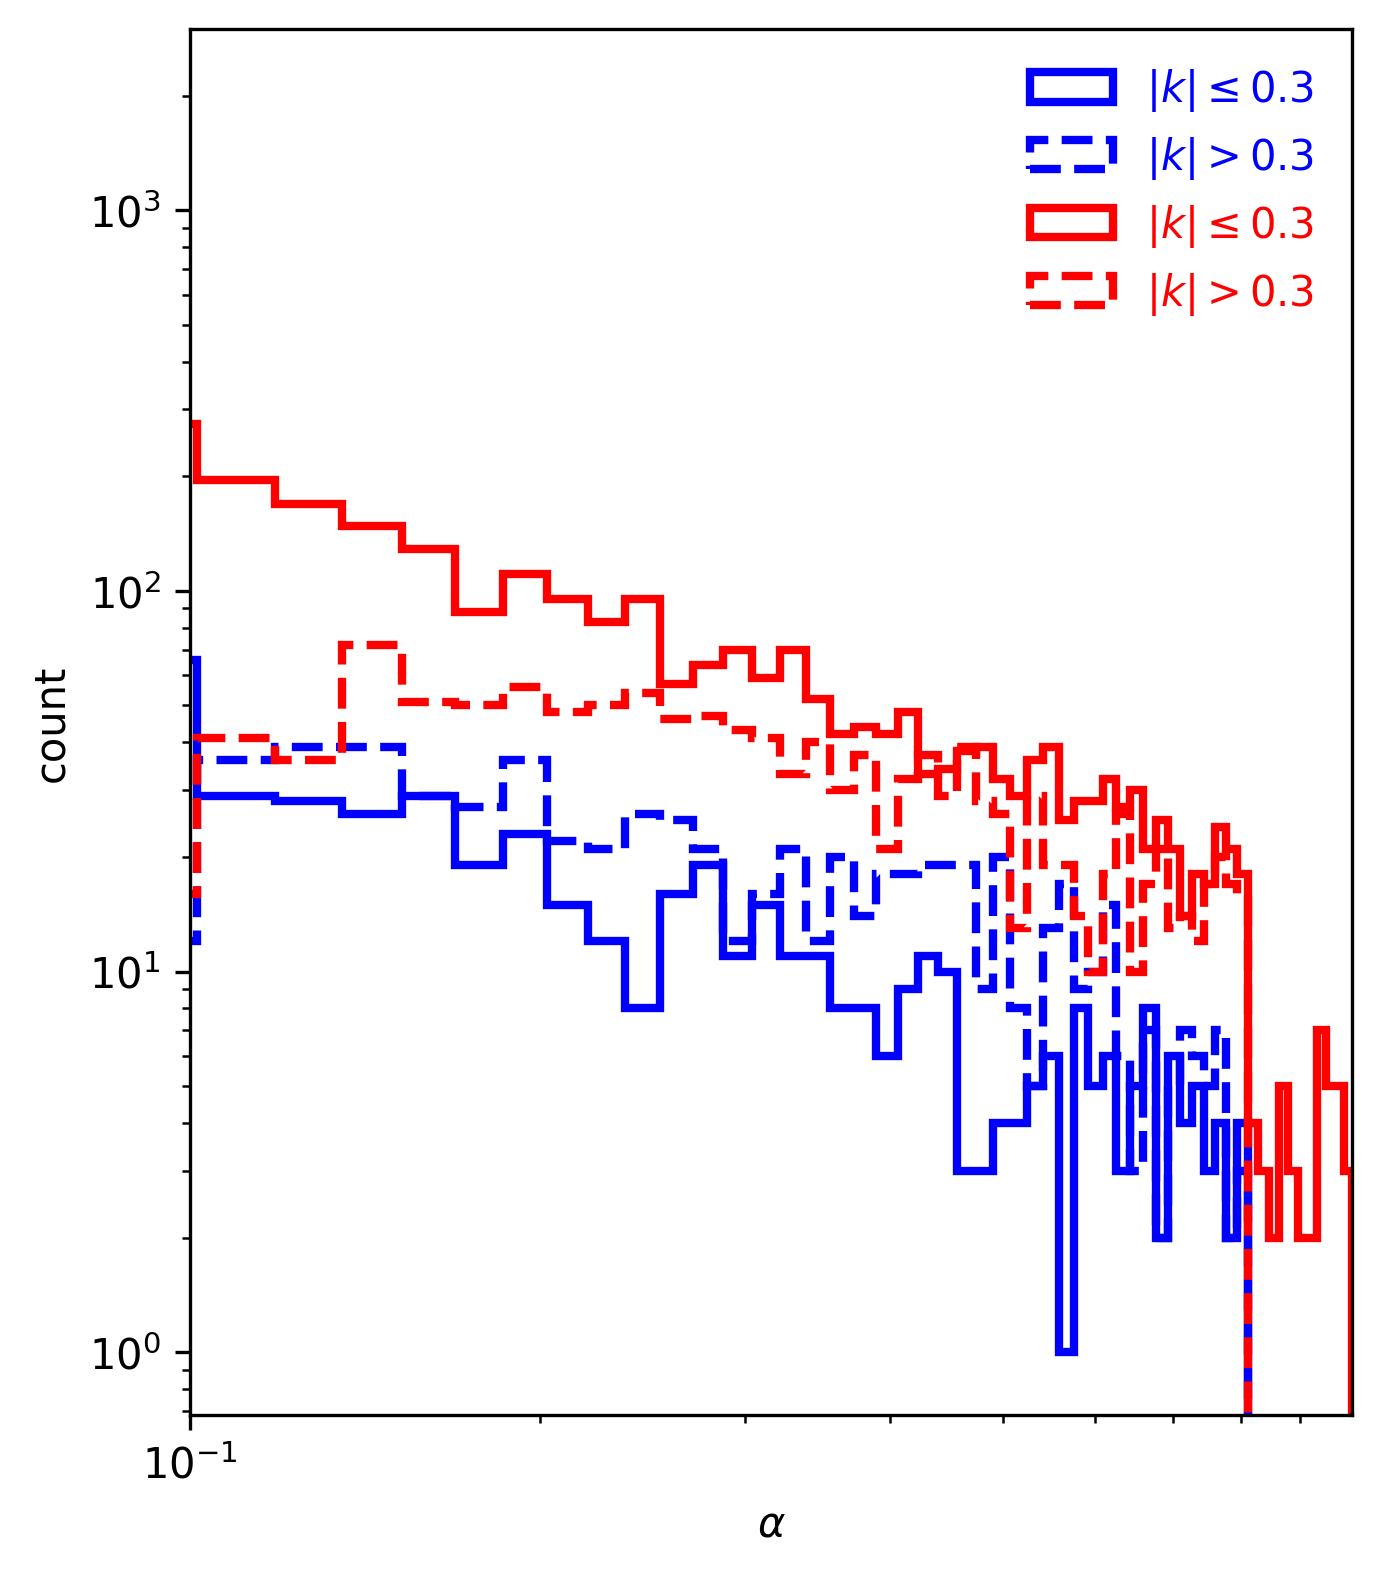
\includegraphics[width=0.6\textwidth]{Figures/Histograms/histogram_alpha.png}
    \caption{Histograms for proportionality constant $\alpha = \langle M_A \rangle^2$ of events identified via GS analysis. For this histogram, blue lines are solar wind events, and red lines are magnetosheath events. Solid lines represent events with a Wal\'en slope $|w|\leq 0.3$ and dashed lines represent events with $|w|> 0.3$.}
    \label{fig:histogram-alpha}
\end{figure}

%Table \ref{tab:walenTest-table} summarizes the classification of the events with the Wal\'en test slope, which further distinguishes traditional magnetic flux rope configurations and Alfv\'enic structures.


%%%%%%%%%%%%%%%%%%%%%%reconstructions%%%%%%%%%%%%%%%%%%%%%%
Figures \ref{fig:reconstruction-Nov2019} and \ref{fig:reconstruction-June2009} are examples of the reconstruction of 2D cross-sections of selected flux rope events, both in the magnetosheath. These were reconstructed using the PyGS package. The black lines indicate the transverse magnetic field lines, and the color background indicates the axial field lines $B_z$ with the strength denoted by the color bar. The flux rope structure is confirmed by the closed field lines region and unipolar $B_z$. The white dot indicates the maximum $B_z$. The white arrows denote the transverse field lines ($B_t$) along the path of the spacecraft ($y=0$), and the green arrows along this path denote the remaining flow velocity. The white contour indicates the area of the reconstruction done from spacecraft data, while the area outside the white contour is reconstructed from extrapolation. The associated time series are displayed below the event reconstructions. The event in Figure \ref{fig:reconstruction-Nov2019} has a Wal\'en slope of -0.09, and the event in Figure \ref{fig:reconstruction-June2009} has a Wal\'en test slope of 0.002. This indicates that the structures are static, where the remaining flow vectors (green) along the spacecraft path in the cross-section have little alignment with the transverse magnetic field line vectors (white arrows). The closed, transverse field lines, and the $B_t$ vectors along the spacecraft path show that the reconstruction in Figure \ref{fig:reconstruction-Nov2019} is a right-handed event, while the structure in Figure \ref{fig:reconstruction-June2009} is a left-handed flux rope. The maximum $B_z$ of the structure in Figure \ref{fig:reconstruction-Nov2019} is 11.85 nT, and that of the structure in Figure \ref{fig:reconstruction-June2009} is 18.21 nT. 

Figure \ref{fig:reconstruction-quasistatic} shows the reconstruction of a quasi-static event in the magnetosheath. It has a much larger scale size ($\sim 5 R_E$) than those in the magnetosheath ($\lesssim 1 R_E$). The Wal\'en test slope of this event is 0.399, which meets the $|k| > 0.3$ threshold.
%It can be seen that the structure has a considerable remaining flow, as indicated by the size of the green arrows. % B_z = 41.19 nT

% \begin{figure}
%     \centering
%     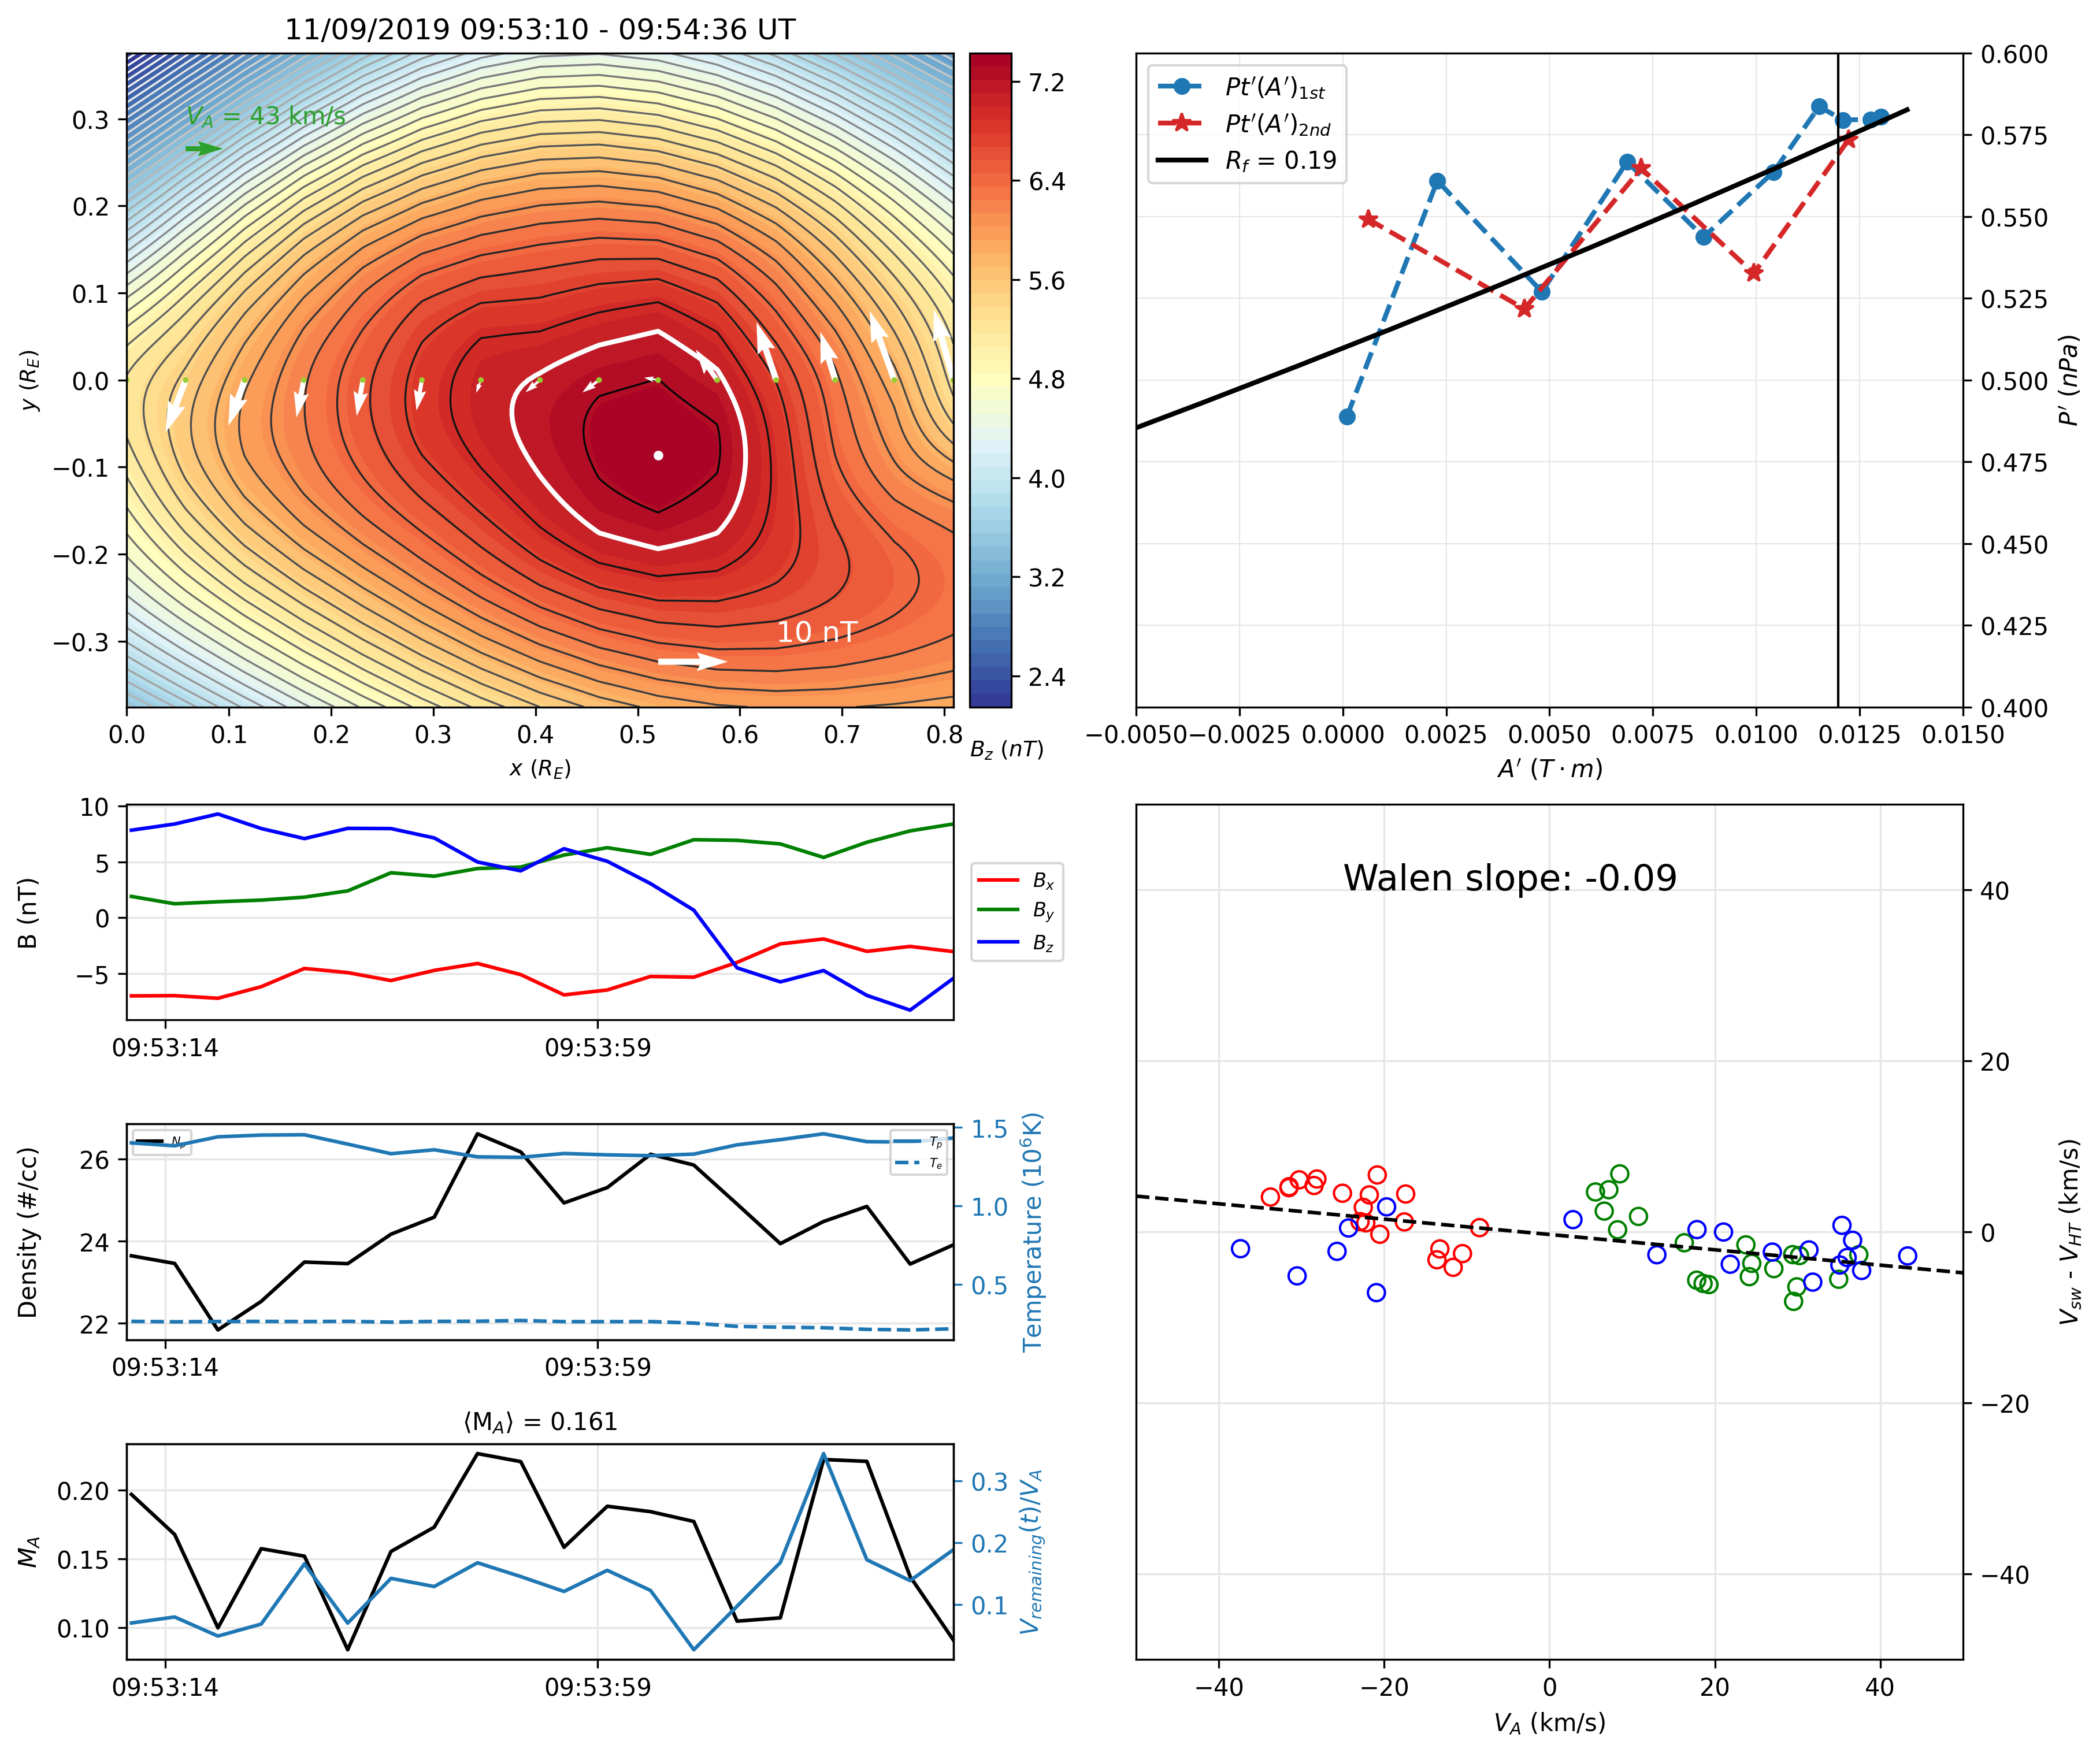
\includegraphics[width=\textwidth]{Reconstructions/timeseries_walenTest_20191109_20191110.png} % in GSE
%     \caption[GS event reconstructions]{GS-based reconstruction of an event 9:53:10-9:54:36 UT on 9 November 2019. Top left: 2D cross-section, with $\hat{x}_{GSE}=[0.890, 0.268, 0.369]$, $\hat{y}_{GSE}=[0.142, 0.605, -0.784]$, $\hat{z}_{GSE}=[-0.433, 0.750, 0.500]$. Bottom left: Associated time series data for MMS-1 in the magnetosheath during this period. Top right:  $P_t'(A')$ vs. $A'$ curve for this event. Bottom right: Wal\'en relation for this event.}
%     \label{fig:reconstruction-Nov2019}
% \end{figure}

\begin{figure}
    \centering
    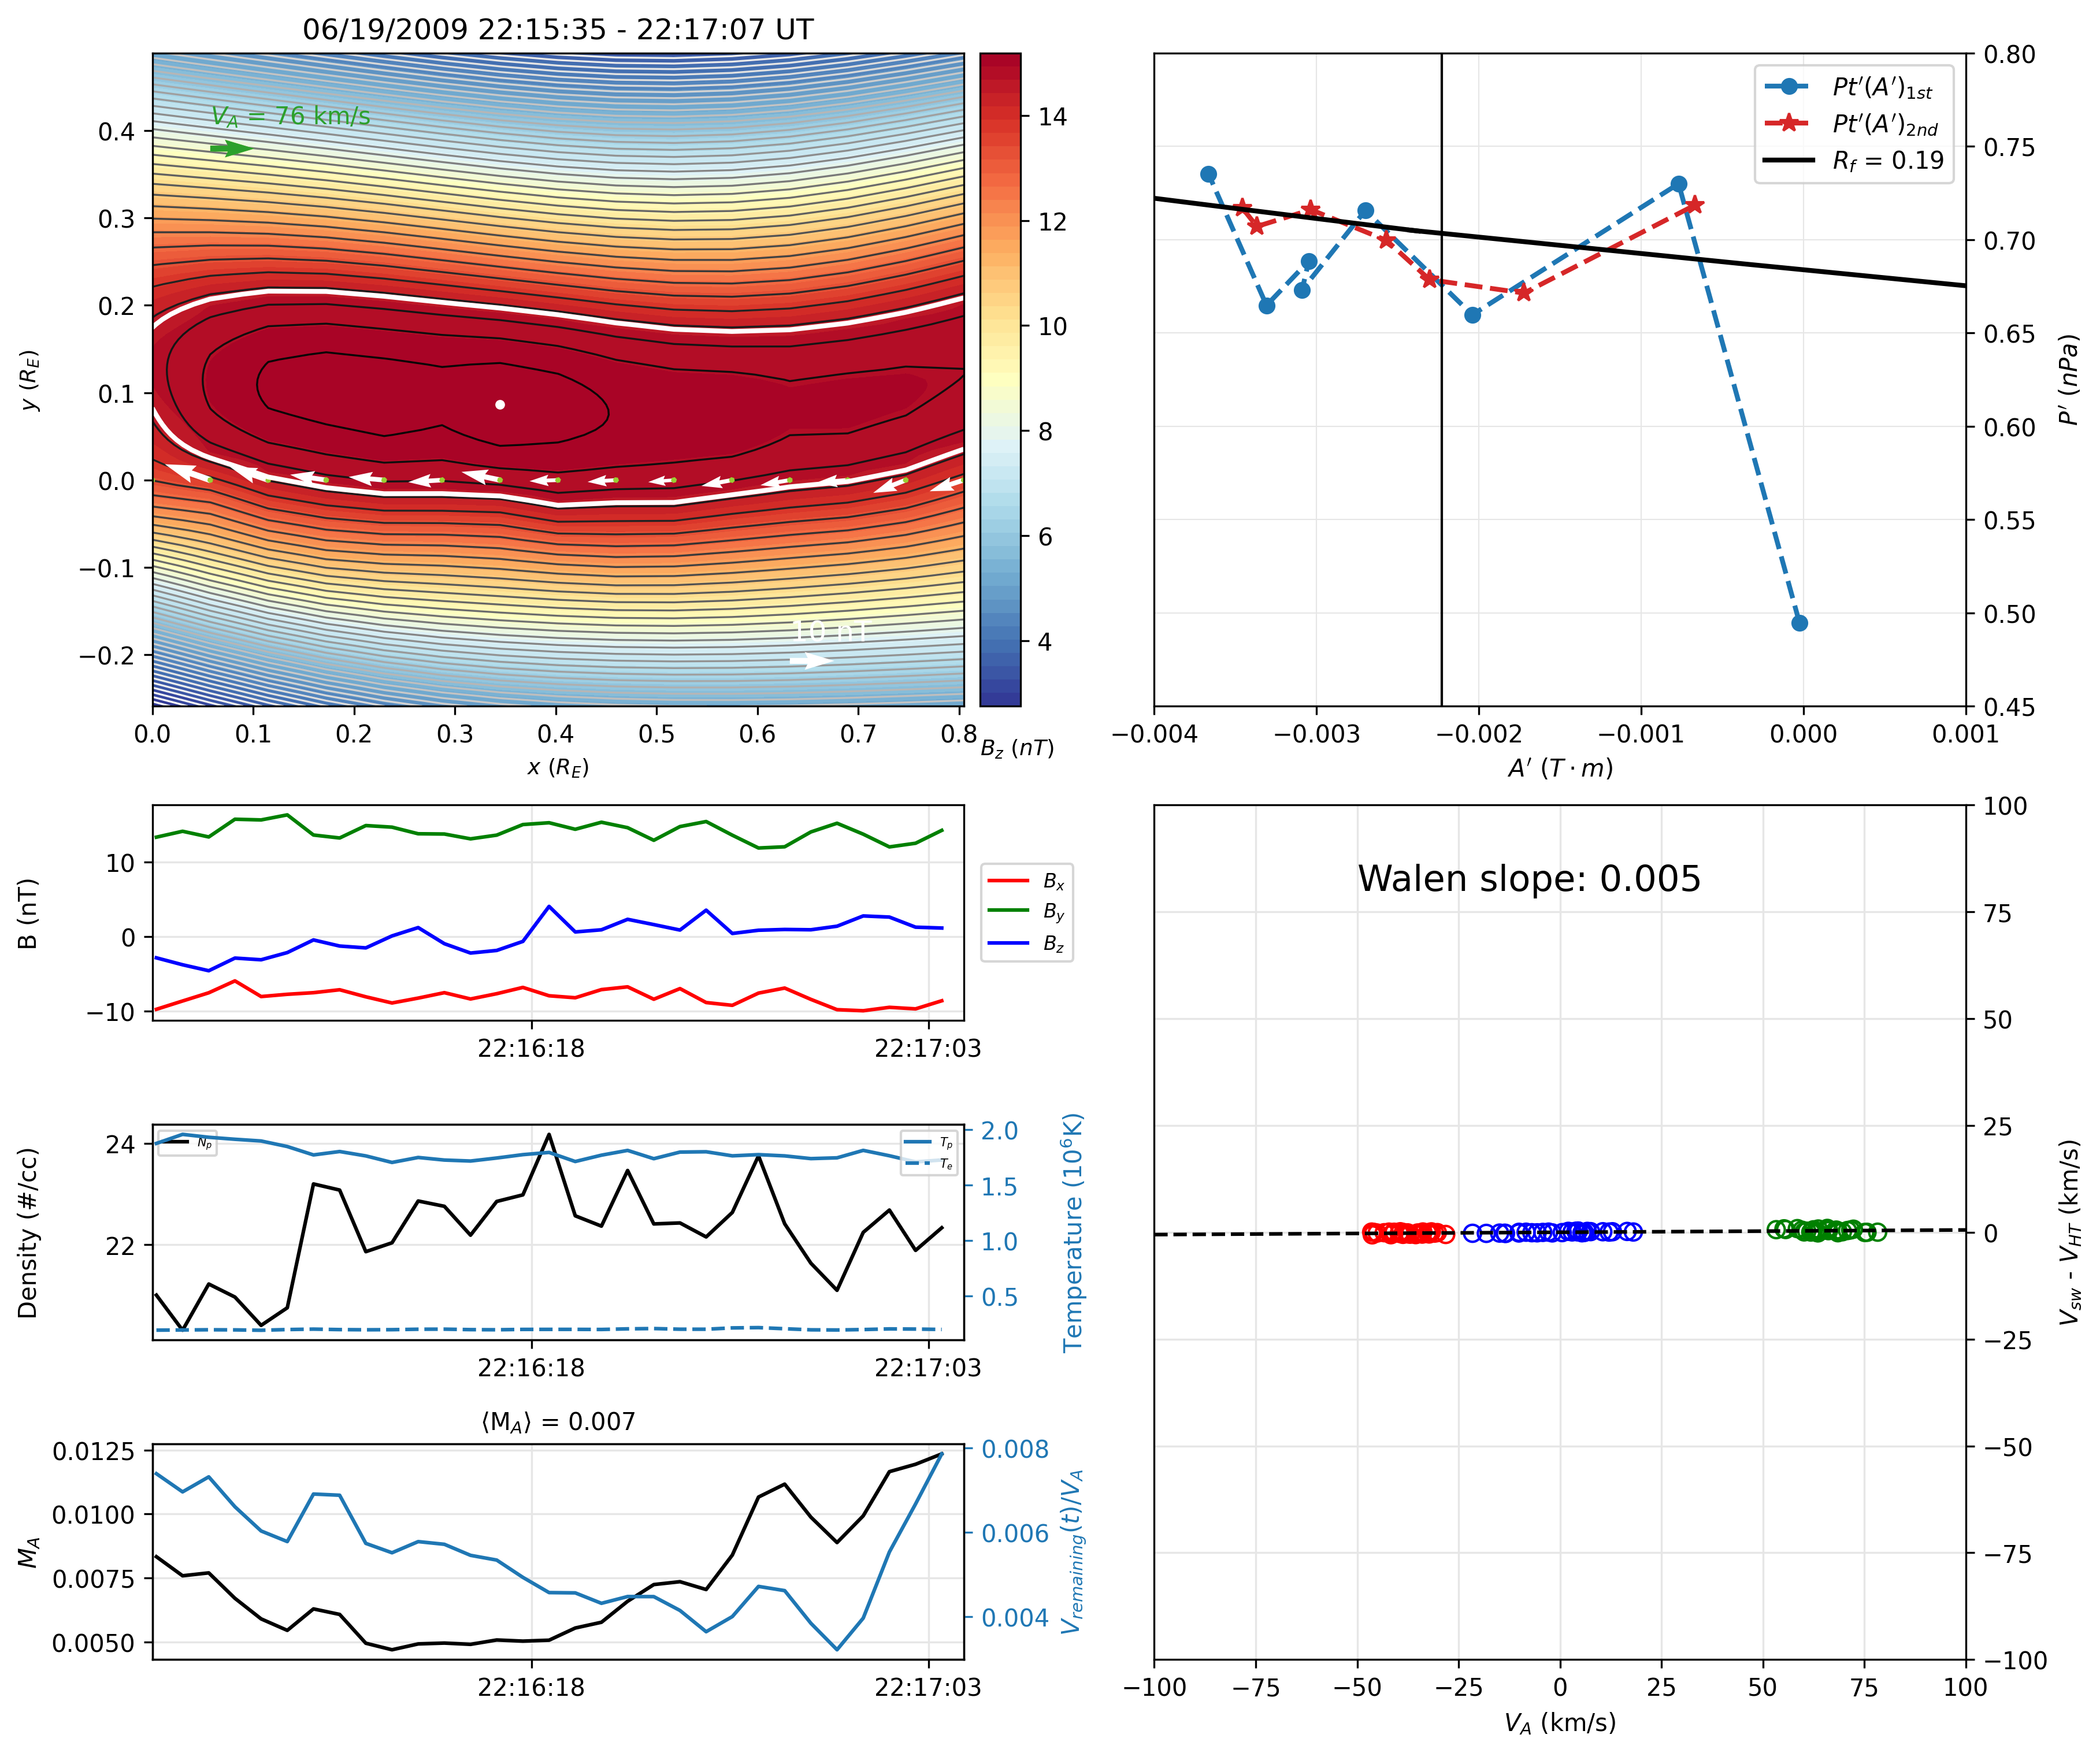
\includegraphics[width=\textwidth]{Reconstructions/timeseries_walenTest_20090619_20090621.png} % in GSE
    \caption[GS event reconstructions]{GS-based reconstruction of an event from 22:15:35-22:17:07 UT on 19 June 2009. Top left: 2D cross-section, with $\hat{x}_{GSE}=[0.761, -0.103, 0.640]$, $\hat{y}_{GSE}=[0.628, 0.365, -0.688]$, $\hat{z}_{GSE}=[-0.163,0.925,0.342]$. Bottom left: Associated time series data for THM-C in the magnetosheath during this period. Top right: $P_t'(A')$ vs. $A'$ curve for this event. Bottom right: Wal\'en relation for this event.}
    \label{fig:reconstruction-June2009}
\end{figure}

%{Reconstructions/stacked_walenTest_20220219_20220220.png}
%\caption[GS event reconstructions]{GS-based reconstruction of an event on 12:52:43-12:58:12 UT on 2 February 2019. Top: 2D cross-section, with $\hat{z}=[0.163,-0.925,-0.342]$. Middle: Wal\'en slope for this event. Bottom: $P_t'$ vs. $A'$ curve for this event.}

% \begin{figure}
%     \centering
%     \includegraphics[width=0.49\textwidth]{Reconstructions/stacked_walenTest_20191109_20191110.png}
%     \includegraphics[width=0.48\textwidth]{Reconstructions/stacked_20090619_20090621.png} % in GSE
%     \caption[GS event reconstructions]{Left: GS-based reconstruction of an event 9:53:10-9:54:36 UT on 9 November 2019. Top: 2D cross-section, with $\hat{x}_{GSE}=[0.890, 0.268, 0.369]$, $\hat{y}_{GSE}=[0.142, 0.605, -0.784]$, $\hat{z}_{GSE}=[-0.433, 0.750, 0.500]$. Bottom: Associated time series data for MMS-1 in the magnetosheath during this period. Right: GS-based reconstruction of an event from 22:15:35-22:17:07 UT on 19 June 2009. Top: 2D cross-section, with $\hat{x}_{GSE}=[0.761, -0.103, 0.640]$, $\hat{y}_{GSE}=[0.628, 0.365, -0.688]$, $\hat{z}_{GSE}=[-0.163,0.925,0.342]$. Bottom: Associated time series data for THM-C in the magnetosheath during this period.}
%     \label{fig:reconstruction}
% \end{figure}



%%%%%%%%%%%%%%%%%%%%%%%%%%%%%%%%%%%%
\begin{figure}
    \centering
    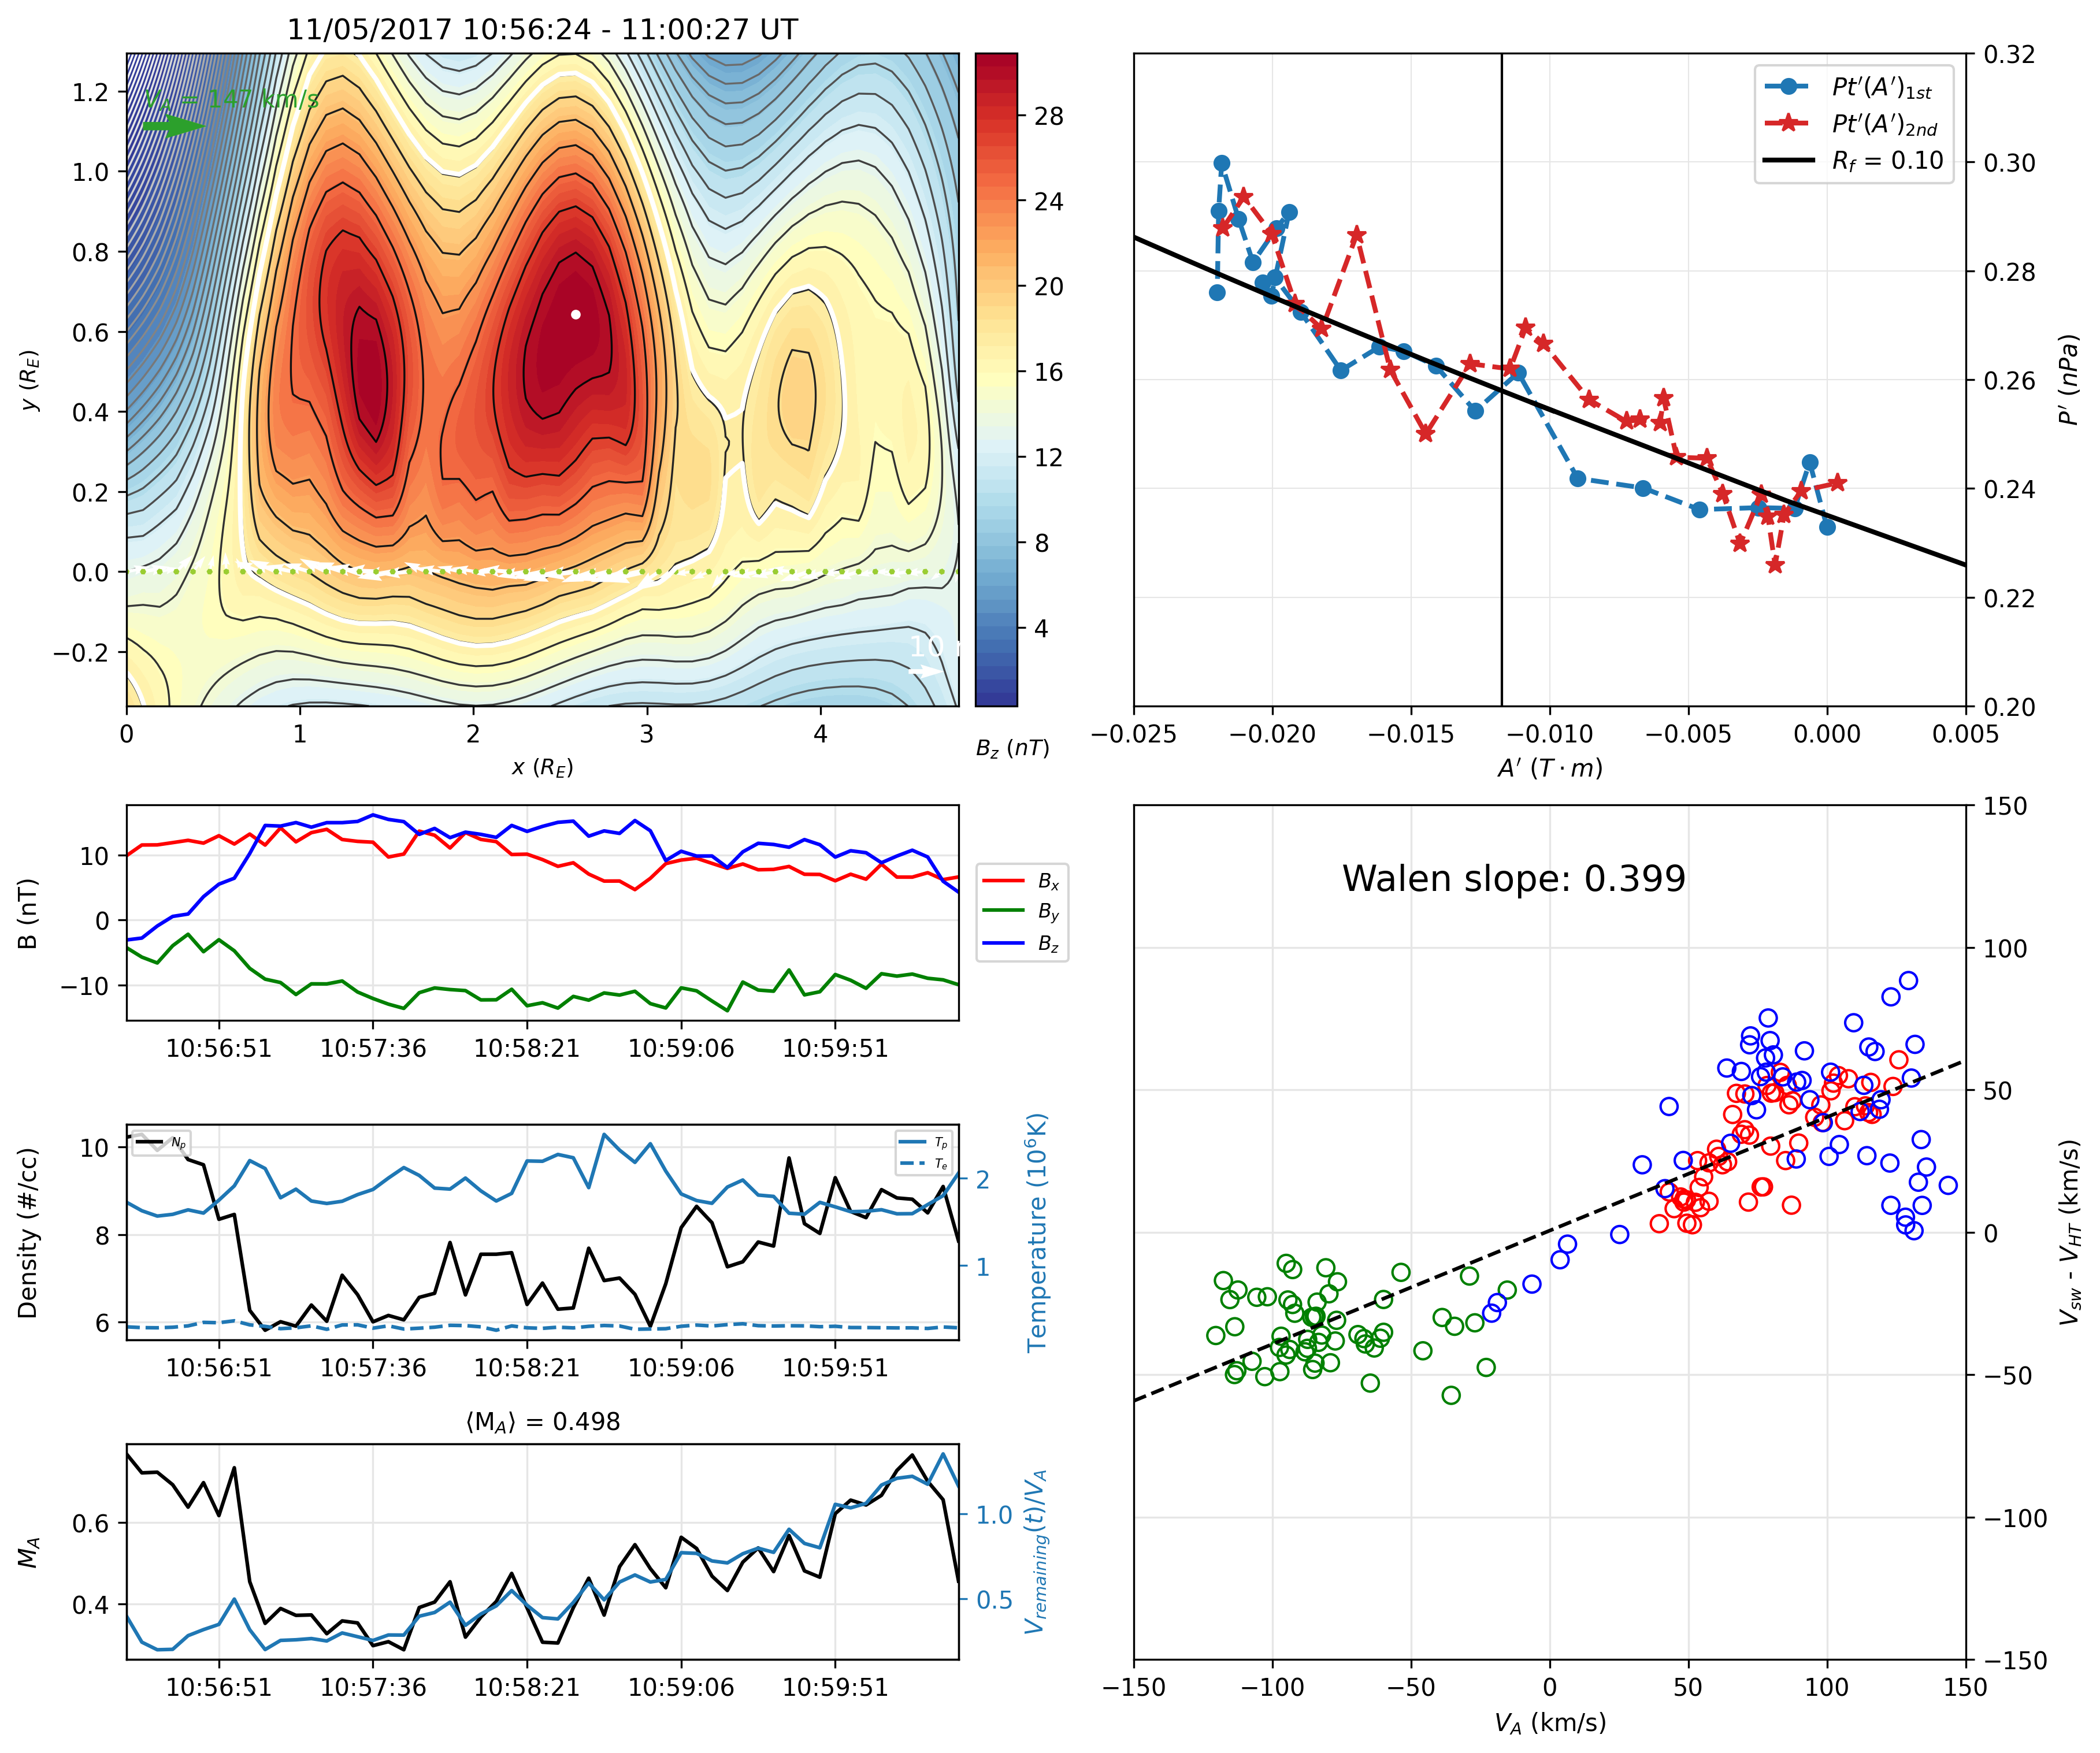
\includegraphics[width=\textwidth]{Reconstructions/timeseries_walenTest_20171105_20171106.png}
    \caption[GS event reconstructions]{GS-based reconstruction of an event on 10:56:24-11:00:27 UT on 05 November 2017 in the magnetosheath from MMS-1. Top left: 2D cross-section, with $\hat{x}_{GSE}=[0.409, -0.029, -0.912]$, $\hat{y}_{GSE}=[0.561, 0.796, 0.226]$, and $\hat{z}_{GSE}=[0.720, -0.604, 0.342]$. Bottom left: Associated time series data for MMS-1 in the magnetosheath during this period. Top right: $P_t'(A')$ vs. $A'$ curve for this event. Bottom right: linear regression of the remaining flow $V_{rem}$ versus the Alfv\'en velocity $V_A$, with Wal\'en slope for this event being 0.399.}
    \label{fig:reconstruction-quasistatic}
\end{figure}


Figure \ref{fig:wavelet-spectrograms-interval} shows an example of event intervals identified via the wavelet algorithm (with the criteria $|\sigma_m|\geq 0.75$) overlaid the corresponding time series and spectrogram of the reduced magnetic helicity in the magnetosheath during 9 November 2019. There are 11 events identified by the wavelet algorithm during this 3 hour period. The duration of these events range from 1 minute to 32.29 minutes, with an average duration of 9.913 minutes. The average maximum magnetic field of the events is 12.23 nT. The average absolute maximum (normalized) magnetic helicity of these 11 events is 0.83. 6 events in this period have $|\sigma_c|\leq 0.3$, and one of those events has $\sigma_r<0$. Of remaining 5 events, none have $\sigma_r<0$.


\section{Conclusions \& Summary}
As a subsection of the analysis, a coordinated analysis between the magnetosheath and solar wind over $\sim$250 hours was performed in order to compare simultaneous observations. 

We find that in the magnetosheath, the magnetic structures identified seem to be compressed relative to the structures in the solar wind. The distributions of the scale sizes and durations of the events shows a linear trend with more, shorter (in duration and size) events in the magnetosheath than in the solar wind. From the GS-based method, we were able to see that the helicity density and poloidal flux were greater in the magnetosheath; these parameters would indicate more compact, twisted structures. From the $z$-axes, we find that the orientation of the polar angle sees a significant change from the solar wind to the magnetosheath: whereas the peak in the distribution of polar angles in the solar wind is around 60-70 degrees, the magnetosheath distribution separates into two peaks, with an almost 180 degree separation. With a wider distribution of polar angles, the magnetic structures in the magnetosheath seem to be less uniform in nature.

\begin{enumerate}
    \item The GS-based reconstruction-based algorithm identifies events with a broader range of cross helicity values than with wavelet analysis.
    \item Static structures were more dominant in both the solar wind and magnetosheath, but there was a higher percentage of quasi-static structures identified in the magnetosheath than in the solar wind. %~10\%
    \item The coordinated analysis shows a direct comparison of the events identified in the magnetosheath and solar wind from simultaneous observations. These results augment the overall analysis, showing trends that align with the extended list.
    \item The identifying spacecraft typically moves through the structures in the magnetosheath in a much more oblique manner when identified with the GS-based method, than when structures are identified in the solar wind.
    \item Identified structures in the magnetosheath (broadly defined as flux ropes with vortical flows) were likely elongated in the downstream flow direction.
\end{enumerate}